\section{Agent-Coordinated Task-Level Operation}
\label{sec:closed-loop-operation}

\begin{figure*}[!t]
\centering
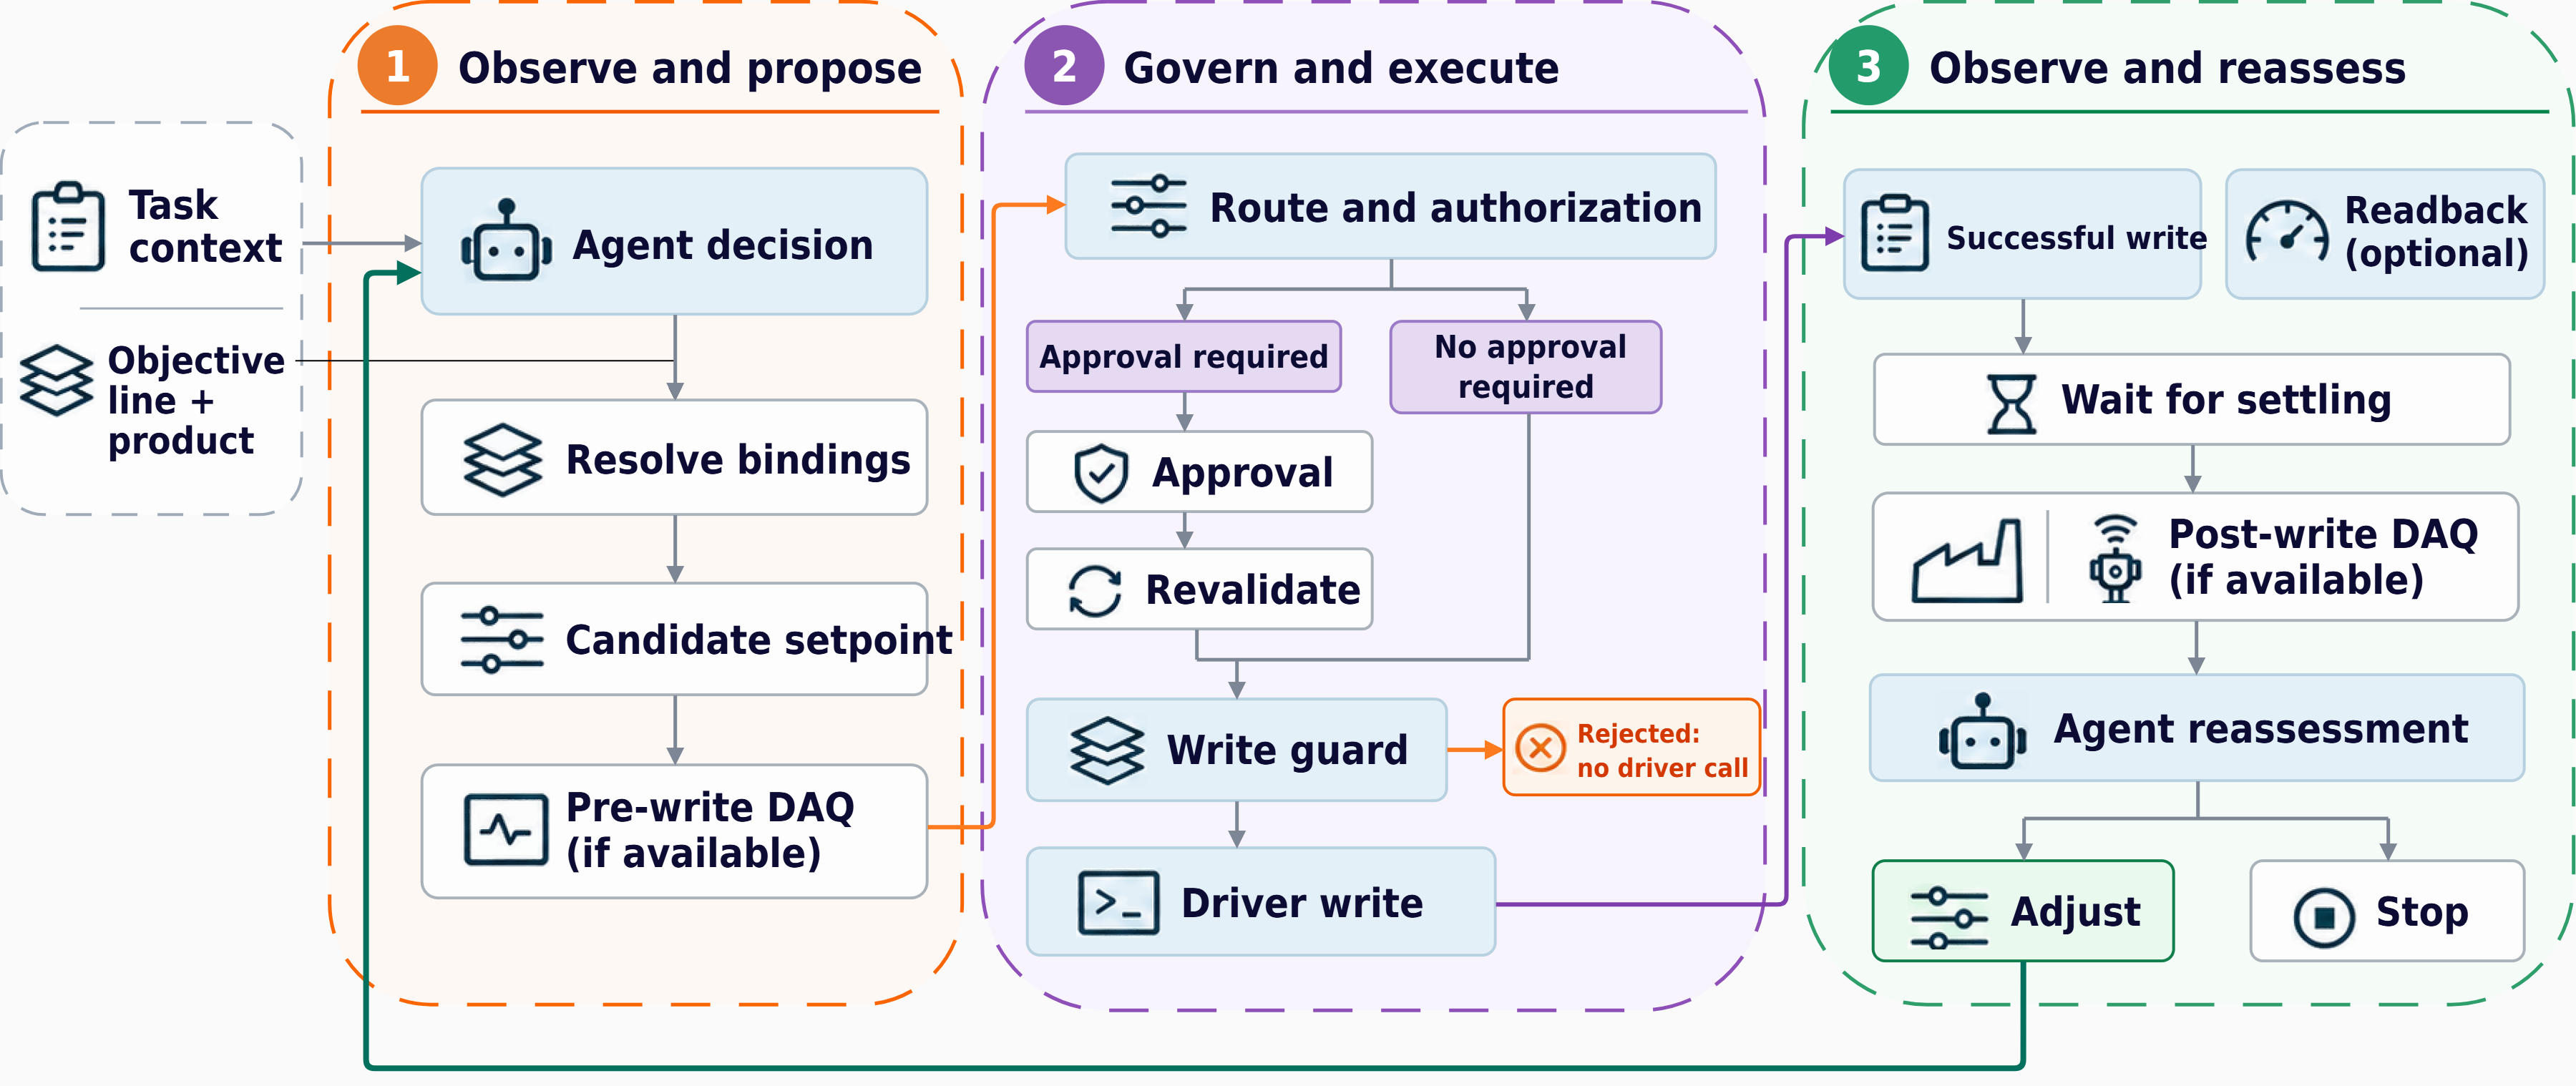
\includegraphics[width=\textwidth]{resources/fig3.png}
\caption{Intended task-mediated acquisition-to-reassessment flow, not a recorded run. The agent uses earlier observations (not shown); pre-write DAQ is an optional subsequent read. Route checks precede dispatch, and Fig.~\ref{fig:hitl} shows the omitted approval-denial path. ``Successful write'' in the diagram denotes reported command success, not verified actuation. A driver error may leave device state uncertain. Optional readback and later DAQ observations answer different questions: whether the setpoint matched and what the process subsequently did.}
\label{fig:agent-loop}
\end{figure*}

Fig.~\ref{fig:agent-loop} follows one intended task-mediated turn. Entry dispatch first establishes the caller, channel, and applicable policy; the route handler then resolves the operation's bindings and applies write-specific checks. The task supplies an objective and production context; the agent reads configured observations, assesses the gap to the objective, and proposes an adjustment. For single-node exploration, \texttt{optimization\_explore} resolves the control node from \texttt{control\_node\_id} or its binding, and resolves the DAQ target from an explicit ID or the agent's DAQ binding. In goal mode, a lead agent may decompose the objective and delegate this step as a worker subtask. The walkthrough is distinct from the scripted \texttt{recipe\_trial} contrast in Section~\ref{sec:eval-optimization}.

The operation resolves the applicable limit profile and control binding, then reads the stored value as $u_0$; this is not necessarily a fresh readback. The agent combines this state with its objective and direction. If direction is omitted, the operation defaults to an upward adjustment; otherwise $s\in\{-1,+1\}$. For a step $\Delta u$, it forms
\begin{equation}
 u^{*}=\operatorname{clip}\!\left(u_0+s\Delta u,\,u_{\min},\,u_{\max}\right).
 \label{eq:optimization-candidate}
\end{equation}
Clipping forms a proposal within configured tuning bounds (or node bounds if absent); it neither authorizes the write nor guarantees admission under Eq.~(\ref{eq:admission}). The effective step comes from the explicit argument, the binding's tuning step, the scene's maximum step, or one twentieth of the node range, in that order.

The operation resolves the DAQ target and checks visibility before the intent enters the governed path; gates added after the reported experiments (identifiability and model--ontology checks) are not exercised in Section~\ref{sec:eval}. If the checks pass, the operation attempts a pre-write DAQ read, whose mean may be unavailable.

A valid candidate enters the governed single-node write path in Algorithm~1: a pre-dispatch denial stops the request before any driver call, whereas a driver-stage error may occur after dispatch has begun, so status alone cannot establish whether the device changed and state must be reconciled before retrying.

After reported command success, the operation waits 10--300~s (45~s default) and attempts another DAQ read. It queries $[t_0-\tau,t_0]$ and $[t_0,t_1]$, with $\tau$ the pre-read window length and $t_1$ the later read time. The implementation sets $t_0$ before the pre-read and any approval wait, not at dispatch, so the second window can include pre-dispatch samples. Earlier code queried trailing 45-s windows instead. The means are descriptive, not causal estimates.

The exploration record stores the target, step, available DAQ means, and write status; the shared path separately records the command outcome and any available readback. The operation then returns an exploration summary. On a later turn, the agent can inspect the returned evidence, choose another step, or stop; iteration always requires a subsequent agent decision.


